\documentclass[11pt,twocolumn]{article}
\usepackage{graphicx}
\usepackage[left=1.80cm, right=1.80cm, top=2.00cm, bottom=2.00cm]{geometry}
\usepackage{amsmath}
\usepackage[colorlinks]{hyperref}
\usepackage[backend=biber]{biblatex}
\usepackage{eurosym}
\usepackage[dvipsnames]{xcolor}
\usepackage{subcaption}
\usepackage{accents}
\usepackage[capitalise]{cleveref}



\addbibresource{main.bib}
\graphicspath{{../figures/}}

\crefname{relation}{Rel.}{Rels.}
\creflabelformat{relation}{(#2#1#3)}
\crefname{constraint}{Constr.}{Constrs.}
\creflabelformat{constraint}{(#2#1#3)}

\setlength\parindent{8pt}

\newcommand{\ie}{\textit{i.e.} }
\newcommand{\eg}{\textit{e.g.} }

\newcommand{\ubar}[1]{\underaccent{\bar}{#1}}
\newcommand{\note}[1]{\textcolor{Orange}{#1}}
\newcommand{\vpad}{\vspace{1mm}}
\newcommand{\hpad}{\hspace{15pt}}

\newcommand{\generation}[1][n]{g_{#1,s,t}}
\newcommand{\generationpotential}{\bar{g}_{n,s,t}}
\newcommand{\generationshare}[1][n]{\omega_{#1,s,t}}
\newcommand{\nodalgeneration}[1][n]{g_{#1,t}}
\newcommand{\capacityGeneration}{G_{n,s}}
\newcommand{\capacityGenerationUpper}{\bar{G}_{n,s}}
\newcommand{\capacityGenerationLower}{\ubar{G}_{n,s}}
\newcommand{\capacityFlow}{F_{\ell}}
\newcommand{\capacityFlowUpper}{\bar{F}_{\ell}}
\newcommand{\capacityFlowLower}{\ubar{F}_{\ell}}
\newcommand{\capexGeneration}{c_{n,s}}
\newcommand{\capexFlow}{c_{\ell}}
\newcommand{\opexGeneration}[1][n]{o_{#1,s}}
\newcommand{\demand}[1][n]{d_{#1,a,t}}
\newcommand{\nodaldemand}[1][n]{d_{#1,t}}
\newcommand{\demandshare}[1][n]{\omega_{#1,a,t}}
\newcommand{\utility}{U_{n,a,t}}
\newcommand{\incidence}[1][n]{K_{#1,\ell}}
\newcommand{\ptdf}[1][n]{H_{\ell,#1}}
\newcommand{\ptdfEqual}[1][n]{\ptdf[#1]^\circ}
\newcommand{\slackflow}{k_{\ell}}
\newcommand{\slack}[1][n]{k_{#1}}
\newcommand{\slackk}[1][n]{k^*_{#1}}
\newcommand{\Slack}{k_{m,n}}
\newcommand{\Slackk}{k^*_{m,n}}
\newcommand{\mulowergeneration}[1][n]{\ubar{\mu}_{#1,s,t}}
\newcommand{\muuppergeneration}[1][n]{\bar{\mu}_{#1,s,t}}
\newcommand{\mulowerflow}{\ubar{\mu}_{\ell,t}}
\newcommand{\muupperflow}{\bar{\mu}_{\ell,t}}
\newcommand{\lmp}[1][n]{\lambda_{#1,t}}
\newcommand{\flow}{f_{\ell,t}}
\newcommand{\cycle}{C_{\ell,c}}
\newcommand{\impedance}{x_\ell}
\newcommand{\cycleprice}{\lambda_{c,t}}
\newcommand{\injection}{p_{n,t}}
\newcommand{\netconsumption}[1][n]{p^{-}_{#1,t}}
\newcommand{\netproduction}[1][n]{p^{+}_{#1,t}}
\newcommand{\selfconsumption}[1][n]{p^{\circ}_{#1,t}}

\newcommand{\totalnetconsumption}{p^{-}_{t}}
\newcommand{\totalnetproduction}{p^{+}_{t}}
\newcommand{\totalselfconsumption}{p^{\circ}_{t}}

\newcommand{\lagrangian}{\mathcal{L}}

\newcommand{\allocatePeer}[1][m \rightarrow n]{A_{#1,t}}
\newcommand{\allocateFlow}[1][n]{F_{#1,\ell,t}}
\newcommand{\allocateTransaction}[1][m \rightarrow n]{A_{#1,\ell,t}}
\newcommand{\allocateCapexGeneration}[1][n]{\mathcal{C}^{G}_{#1,t}}
\newcommand{\allocateCapexFlow}[1][n]{\mathcal{C}^{F}_{#1,t}}
\newcommand{\allocateOpex}[1][n]{\mathcal{O}_{#1,t}}
\newcommand{\allocateEmissionCost}[1][n]{\mathcal{E}_{#1,t}}


\newcommand{\emission}[1][n]{e_{#1,s}}
\newcommand{\emissionPrice}{\mu_{\text{CO2}}}
\newcommand{\megawatthour}{MWh$_\text{el}$}
\newcommand{\totalcost}{\mathcal{TC}}
\newcommand{\totalOpexGeneration}{\mathcal{O}}
\newcommand{\totalOpexFlow}{\mathcal{O}^F}
\newcommand{\totalCapexGeneration}{\mathcal{C}^G}
\newcommand{\totalCapexFlow}{\mathcal{C}^F}
\newcommand{\totalEmissionCost}{\mathcal{E}}

\newcommand{\impactcapexgeneration}{\Phi_{n,s,t}}
\newcommand{\impactcapexflow}{\Phi_{\ell,t}}

%math 
\newcommand{\resultsin}[1]{\hspace{6pt} \bot  \hspace{6pt} #1}
\newcommand{\Forall}[1]{\hspace{10pt} \forall \,\, #1 }
\newcommand{\pdv}[2]{\frac{\partial #1}{\partial #2}}

\begin{document}


\title{From Linear Optimization to Transmission Cost Allocation}
\author{F. Hofmann. T. Brown}

\maketitle

\begin{abstract}
Maximizing the welfare of all market participants within a power system is a common approach in energy system modelling. It leads to perfectly scheduled operations of generators and ... 
\end{abstract}




% In the following, we show how Flow Allocation (FA) can be used for decomposing Locational Marginal Prices (LMP) in a linear optimized power system. We begin by revising the fundamentals of the Power Transfer Distribition Factors (PTDF) and the role of the slack, which plays a key role for FA. This will lead us to a generalized form of peer-to-peer allocations and transmission usage allocations based on the choice of slack. In a second step, we breakdown the full Lagrangian of a cost-optimization for a network with transmission and generation capacity expansion. By taking into account sensitivities of the flow with respect to changes in the nodal generation, we are able to derive a cost allocation which directly links to FA.  

% \section{Introduction}

\subsubsection*{Nomenclature}

\begin{table}[h]
	\centering
	\begin{tabular}{ll}
        $\lmp$ & Locational Market Price at bus $n$ and  \\ & time step $t$ in \euro/MW \vpad \\
        $\demand$ & Electric demand per bus $n$, demand type $a$, \\ & time step $t$ in MW  \vpad \\
        $\generation$ & Electric generation per bus $n$, carrier $s$, \\ & time step $t$  in MW \vpad \\
        $\flow$ & Active power flow on line $\ell$, \\ & time step $t$ in MW   \vpad \\
        $\opexGeneration$ & Operational cost (OPEX) in \euro/MW \vpad \\
        $\capexGeneration$ & Capital Expenditure (CAPEX) in \euro/MW \vpad \\
        $\capexFlow$  & CAPEX per transmission line $\ell$ in \euro/MW  \vpad \\
        $\capacityGeneration$ & Generation capacity in MW \vpad \\
        $\capacityFlow$ & Transmission capacity in MW \vpad \\
        $\incidence$ & Incidence matrix \vpad 
	\end{tabular}
\end{table}

\section{Economic Context}

In long-term operation and investment planning models, the total costs $\totalcost$ of a power system include all operational expenditures (OPEX) $\totalOpexGeneration$ and capital expenditures (CAPEX) $\totalCapexGeneration$ and $\totalCapexFlow$ for production  and transmission respectively, thus
\begin{align}
  \totalcost &= \totalOpexGeneration + \totalCapexGeneration +  \totalCapexFlow + \text{rest}
  \label{eq:total_cost_terms}
\end{align}
In a network design with minimal $\totalcost$, the Locational Market Price (LMP) describes the marginal price for an incremental increase of electricity demand $\demand$ of any consumer $a$ at bus $n$. It is given by the derivative of the total system cost $\totalcost$ with respect to the local demand $\demand$
\begin{align}
 \lmp = \pdv{\,\totalcost}{\,\demand}
 \label{eq:total_cost_derivative}
\end{align}
This leads to a nodal pricing where over the span of optimized timesteps $t$, the system costs are totally payed back by the consumers 
\begin{align}
 \totalcost &=  \sum_{n,a,t} \lmp \, \demand
 \label{eq:total_cost_sum}
\end{align}
% 
\begin{figure}[h]
\centering
 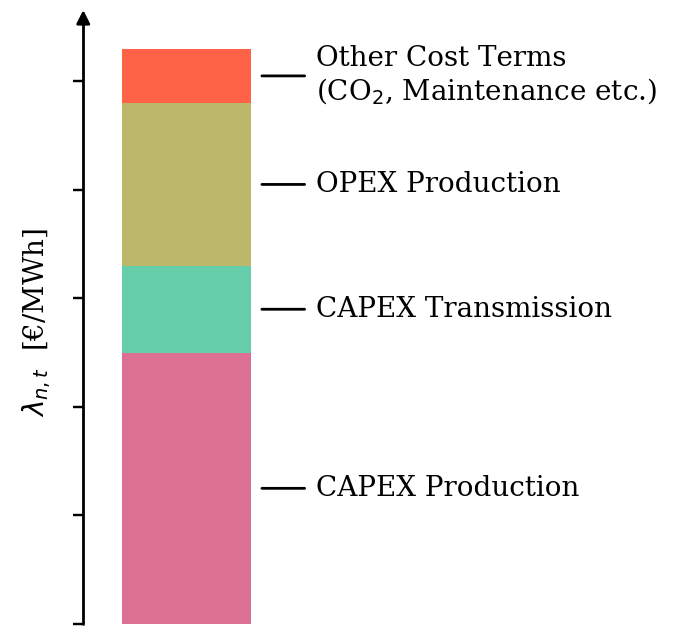
\includegraphics[width=.8\linewidth]{price_decomposition.png}
 \caption{Schematic decomposition of the Locational Market Price $\lmp$. In power system model with optimal long-term operation and planning, the total system costs $\totalcost$ split into different cost terms, \textit{i.e} OPEX and CAPEX for production and transmission and possibly other expenditures. As $\,\totalcost$ is fully payed by the consumers, each LMP $\lmp$ can be decomposed into cost terms compensating the different expenditures at timestep $t$.}
 \label{fig:price_decomposition}
\end{figure}

% 
As a direct consequence of \cref{eq:total_cost_terms,eq:total_cost_derivative,eq:total_cost_sum}, the LMP splits into different cost terms assigned to OPEX and CAPEX for production and transmission and eventual other expenditures. We schematically show this behaviour in \cref{fig:price_decomposition}. 
Extensive investigations of the LMP as done in \cite{schweppe_spot_1988} already showed this connection however leave the question open how the costs are allocated among the components. In the following we will show how the above presented cost decomposition is extended to full peer-to-peer cost allocation including all network components. 



\section{Mathematical Theory}



\subsection{Power Transfer Distribition Factors and Flow Allocation}


In linear power flow models, the Power Transfer Distribition Factors (PTDF) $\ptdf$ determine the changes in the flow on line $\ell$ for one unit (typically one MW) of net power production at bus $n$. Thus for a given production $\generation$ and demand $\demand$, they directly link to the the resulting flow on each line, 
\begin{align}
 \flow  =   \sum_n \ptdf  \left( \nodalgeneration- \nodaldemand \right)    
 \label{eq:flow_from_ptdf}
\end{align}
where $\nodalgeneration = \sum_s \generation$ and $\nodaldemand = \sum_a \demand$ combine all generators $s$ and all comsumers $a$ attached to $n$.
The PTDF have a degree of freedom: The slack $\slack$ denotes the contribution of bus $n$ to balancing out total power excess or deficit in the system. It can be dedicated to one bus, a sinlge ``slackbus``, or to several or all buses. The choice of slack modifies the PTDF according to 
\begin{align}
 \ptdf\left( \slack[m]\right)  = \ptdfEqual - \sum_m \ptdfEqual[m]  \, \slack[m]
 \label{eq:ptdf_slacked}
\end{align}
where $\ptdfEqual$ denote the PTDF with equally distributed slack.
When bus $n$ injects excess power, it has to flow to the slack; when bus $n$ extract deficit power, it has to come from the slack. Summing over all ingoing and outgoing flow changes resulting from a positive injection at $n$ yields again the slack 
\begin{align}
\sum_\ell \incidence[m] \, \ptdf =  \delta_{m,n} - \slack[m] 
\label{eq:slack}
\end{align}
Note that $\delta_{m,n}$ on the right hand side represents the positive injection at $n$.
% As shown above, the choice of slack $\slack[m]$ decides on the generators and lines to which power imbalances are distributed to. 
Established flow allocation schemes [cite] haved used this degree of freedom in order to allocate power flows and exchanges to market participants. Under the assumption that consumers account for all power flows in the grid, the slack is set to $\slack^*$ such that 
\begin{align}
 \flow  = - \sum_n \ptdf\left( \slackk[m]\right) \, \nodaldemand  
 \label{eq:flow_from_demand}
\end{align}
With such a choice the flow can be reproduced from the demand-side of the system only. Now each term in the sum on the right hand side stands for the individual contribution of consumers at node $n$ to the network flow $\flow$. In other words, each nodal demand $\nodaldemand$ induces a subflow originating from the slack $\slackk$ which all together add up to $\flow$. These subflows, in turn, can be further broken down to contributions for each bus $m$ in the slack, such that we get the subflow of individual $m \rightarrow n$ relations, that is 
\begin{align}
 \allocateTransaction = \left(  \ptdfEqual[m] - \ptdfEqual \right) \slackk[m] \, \nodaldemand
 \label{eq:allocate_transaction}
\end{align}
% 
It indicates the flow on line $\ell$ coming from generators at $m$ and supplying the demand $\nodaldemand$. When summing over all sources $m$ it yields the total subflow induced by $\nodaldemand$, the same term as in the sum on the right hand side in \cref{eq:flow_from_demand}; 
% \begin{align}
% \sum_m \allocateTransaction = -\ptdf\left(\slackk[m] \right) \,  \nodaldemand
% \end{align}
when summing over all sources and sinks, it yields again the power flow, thus
\begin{align}
\flow = \sum_{m,n} \allocateTransaction
\label{eq:transaction_sum}
\end{align}
% 
As mentioned before, the consumed power $\nodaldemand$ has to come from the slack $\slackk[m]$. As proofen in \cref{sec:proof_allocate_peer}, for each peer-to-peer relation $m \rightarrow n$, the ``traded`` power $\allocatePeer$  amounts to
\begin{align}
 \allocatePeer &= \slackk[m] \, \nodaldemand 
\label{eq:allocate_peer}
\end{align}
% 
Finally, when summing over all sinks the peer-to-peer trades yield the nodal generation (see \cref{sec:proof_sum_n_allocate_peer}) 
\begin{align}
 \sum_n \allocatePeer = \nodalgeneration[m]
 \label{eq:sum_n_allocate_peer}
\end{align}
and summing over all sources yields the nodal demand 
\begin{align}
 \sum_m \allocatePeer = \nodaldemand
 \label{eq:sum_m_allocate_peer}
\end{align}
which follows from the fact that $\sum_n \slackk = 1$.
Both allocation quantities $\allocatePeer$ and $\allocateTransaction$ can be broken down to generators $s$ or consumers $a$ by multiplying with the nodal production share $\generationshare = \generation/\sum_s \generation$ and the nodal comsumer share $\demandshare = \demand/\sum_a \demand$ respectively. \\


The solution to $\slackk$ follows from combining \cref{eq:allocate_peer,eq:sum_n_allocate_peer}, which sets it to the share of the total production $\slackk = c \, \nodalgeneration$ with $c$ being defined as $c = 1/\sum_n \nodalgeneration$. That leads to the demand $\demand$ of every single consumers $a$ being supplied by all generators $s$ in the network proportional to their gross production $\generation$. However as we discuss in \cref{sec:solution_space_of_the_slack}, the solution space can be extended to an individual slack for each node $\Slackk$.



\subsection{Network Optimisation}

% Maximise $f(x_l)$, with equality constraints $g_i(x_l)$ and inequality constraints $h_j(x_l)$
% 
% \begin{align}
%  \mathcal {L}(x_l,\lambda_i, \mu_j)=f(x_l)-\sum_i \lambda_i \, g_i(x_l) - \sum_j \mu_j \, h_j(x_l)
% \end{align}
% ...
% 

We linearly cost-optimize the capacity and dispatch of a simple power system. 

\begin{align}
    \underset{\generation, \capacityGeneration, \capacityFlow}{\text{min}}
    \left(\sum_{n,s} \capexGeneration \capacityGeneration + \sum_{n, s, t} \opexGeneration \generation + \sum_{\ell} \capexFlow \, \capacityFlow \right) \label{eq:minisation}
\end{align}
subject to following physical constraints. 
\\

The nodal balance constraint ensures that the amount of power that flows into a bus equals the power that flows out of a bus, thus reflects the Kirchhoff Current Law (KCL)
\begin{align}
    \sum_l \incidence \, \flow  - \nodalgeneration + \nodaldemand &= 0 \resultsin{\lmp} \Forall{n,t}
    \label[constraint]{eq:nodal_balance_lin}
\end{align}
Its shadow price mirrors the Locational Marginal Prizes (LMP) $\lmp$ per bus and time step. In a power market this is the \euro/\megawatthour-price which a consumer has to pay. Note that the flow $\flow$ in \cref{eq:nodal_balance_lin} is a passive variable only, given by \cref{eq:flow_from_ptdf}.\\

The generation $\generation$ is constraint to its nominal capacity
\begin{align}
 \generation - \generationpotential \capacityGeneration  &\le 0 \resultsin{\muuppergeneration} \Forall{n,s,t} 
 \label[constraint]{eq:upper_generation_capacity_constraint}\\ 
 - \generation &\le 0 \resultsin{\mulowergeneration} \Forall{n,s,t} 
 \label[constraint]{eq:lower_generation_capacity_constraint}
 \end{align}
where $\generationpotential \in \left[ 0,1\right]$ is the capacity factor for renewable generators. The constraints yield the KKT variables $\muuppergeneration$ and $\mulowergeneration$ which due to complementary slackness,
\begin{align}
\muuppergeneration \left( \generation - \generationpotential \, \capacityGeneration \right)  &= 0  \Forall{n,s,t} 
\label{eq:complementary_slackness_upper_generation} \\
\mulowergeneration  \, \generation &= 0 \Forall{n,s,t}
\label{eq:complementary_slackness_lower_generation} 
\end{align}
are only non-zero if the corresponding constraint is binding. \\


The transmission capacity $\capacityFlow$ limits the flow $\flow$ in both directions, such that 
\begin{align}
 \flow - \capacityFlow &\le 0 \resultsin{\muupperflow} \Forall{\ell,t} 
 \label[constraint]{eq:upper_flow_capacity_constraint} \\
 - \flow - \capacityFlow &\le 0 \resultsin{\mulowerflow} \Forall{\ell,t} 
 \label[constraint]{eq:lower_flow_capacity_constraint}
\end{align}
The yielding KKT variables $\muupperflow$ and $\mulowerflow$ are only non-zero if $\flow$ is limited by the trasmission capacity in positive or negative direction, i.e. \cref{eq:upper_flow_capacity_constraint} or \cref{eq:lower_flow_capacity_constraint} are binding. The complementary slackness 
\begin{align}
 \muupperflow \left( \flow - \capacityFlow \right)  &= 0 \Forall{\ell,t}
 \label{eq:complementary_slackness_upper_flow} \\
 \mulowerflow \left( \flow - \capacityFlow \right) &=  0 \Forall{\ell,t}
 \label{eq:complementary_slackness_lower_flow} 
\end{align}
set the respective KKT for flows staying below the thermal limit to zero. 
\\



\subsection{Allocating Nodal Payments}
\begin{align}
\notag
 & \lagrangian\left(\generation, \flow, \capacityGeneration, \capacityFlow, \boldsymbol{\lambda}, \boldsymbol{\mu} \right)   =   \\  
 \notag
 & \;\;\; \sum_{n,s} \capexGeneration \capacityGeneration + \sum_{n, s, t} \opexGeneration \generation + \sum_{\ell} \capexFlow \, \capacityFlow  \\
 \notag
 &+ \sum_{n,t} \lmp \left(\sum_\ell \incidence \, \flow  - \sum_s \generation + \sum_a \demand  \right)  \\ 
 \notag
 &+ \sum_{\ell,c,t} \cycleprice \, \cycle \, \impedance \, \flow  \\
 \notag
 &+ \sum_{n,s,t} \muuppergeneration \left( \generation - \generationpotential \capacityGeneration \right)  - \sum_{n,s,t} \mulowergeneration \generation  \\
 &+ \sum_{\ell,t} \muupperflow \left( \flow - \capacityFlow \right) - \sum_{\ell,t} \mulowerflow \left( \flow + \capacityFlow \right)     
 \label{eq:full_lagrangian}
\end{align}
% 
where $\boldsymbol{\lambda} = \left\lbrace \lmp, \cycleprice \right\rbrace $ and $\boldsymbol{\mu} = \left\lbrace \muuppergeneration, \mulowergeneration, \muupperflow, \mulowerflow \right\rbrace $ denote the set of related KKT variables. The global maximum of the Lagrangian requires stationarity with respect to all variables. The stationarity of the generation capacity variable leads to 
\begin{align}
 \pdv{\lagrangian}{\capacityGeneration}  = 0 \,\, \rightarrow \,\, 
 \capexGeneration =  \sum_t \muuppergeneration \, \generationpotential  \Forall{n,s}
 \label{eq:capexGeneration_duality}
\end{align}

the stationarity of the transmission capacity to
\begin{align}
 \pdv{\lagrangian}{\capacityFlow} = 0 \,\, \rightarrow \,\, 
 \capexFlow =  \sum_t \left( \muupperflow - \mulowerflow \right) \Forall{\ell}
 \label{eq:capexFlow_duality}
\end{align}


and the stationarity of the generation to 
\begin{align}
 \pdv{\lagrangian}{\generation} &= 0 \,\, \rightarrow \,\,  
 \opexGeneration =  \lmp - \muuppergeneration + \mulowergeneration \Forall{n,s} \label{eq:opex_duality}
\end{align}
Solving \cref{eq:opex_duality} for the $\lmp$, leads to our first representation for Locational Market Price, which we will refer to as the ``Island Solution``,
\begin{align}
\lmp  =  \opexGeneration + \muuppergeneration - \mulowergeneration \Forall{n,s,t}
\label{eq:lmp1}
\end{align}
It connects the LMP directly with the local operational price and prices for the generation capacity constraint. However, we can derive a second representation for $\lmp$. Starting from the stationarity of the flow
\begin{align}
 0 =& \pdv{\lagrangian}{\flow}  \\
 \notag
 0 =&  \sum_{m,\ell,t} \lmp[m] \, \incidence[m]  + \sum_{\ell} \left( \muupperflow - \mulowerflow \right)  \\
 & +\sum_{\ell,c,t} \cycleprice \, \cycle \, \impedance
\end{align}
and multipying each term with the Power Transfer Distribution Factor $\ptdf$ leaves us with  

\begin{align}
  0 &= \lmp - \sum_m \lmp[m] \, \slack[m]  + \sum_{\ell} \left( \muupperflow - \mulowerflow \right) \ptdf
  \label{eq:lmp_lmp1_reduced}
\end{align}
According to \cref{eq:slack}, the first term splits into the LMP at $n$ and the LMP weighted with the slack. The final term disappears as the $\cycle \, \impedance$ is the kernel of the PTDF $\ptdf$, so $\sum_l \cycle \, \impedance \ptdf = 0$. Solving \cref{eq:lmp_lmp1_reduced} for $\lmp$ and replacing $\lmp[m]$ of the right hand side with the expression of the Island Solution in \cref{eq:lmp1} leads to 

\begin{align}
\notag
\lmp =&  \sum_m \opexGeneration[m]\, \slack[m]  + \sum_m \left( \muuppergeneration[m] - \mulowergeneration[m] \right) \slack[m] \\
& -\sum_\ell \left( \muupperflow - \mulowerflow\right) \ptdf  \Forall{n,s,t} 
\label{eq:lmp2}
\end{align}
%  
% NOTE: \cref{eq:lmp2} builds a starting point for breaking down the market value (MV) 
% of generator $(m,s)$, defined as
% \begin{align}
%  MV_s = \dfrac{\sum_t \generation \, \lmp}{\sum_t \generation}
% \end{align}
In contrast to the Island Solution in \cref{eq:lmp1}, this representation connects $\lmp$ with all other prices in the system. Moreover, it must hold for any choice of $\slack[m]$ and correspondingly decomposes the LMP to operational prices $\opexGeneration[m]$ and prices for capacity bounds for generators and transmission lines. When setting the slack to $\slackk[m] = c \, \generation[m]$, the LMP decomposes to prices of generators proportional to their production plus an extra term for the transmission usage. This directly links to the flow allocation presented above. Multiplied with the nodal demand $\nodaldemand$ the left hand side of \cref{eq:lmp2} turns into the total payment of $n$ and the right hand side into the different payment allocations, 
\begin{align}
 \lmp \, \nodaldemand = \allocateOpex + \allocateCapexGeneration + \allocateCapexFlow \Forall{n,t}
 \label{eq:lmp_allocation}
\end{align}
which we define as  
\begin{align}
 \allocateOpex &= 
 \sum_{m,s} \opexGeneration[m] \, \generationshare[m] \, \allocatePeer 
\label{eq:allocate_opexGeneration}\\
 \allocateCapexGeneration &= 
 \sum_{m,s} \muuppergeneration[m] \, \generationshare[m] \, \allocatePeer
\label{eq:allocate_capexGeneration} \\
 \allocateCapexFlow &=  
 \sum_{m,\ell} \left( \muupperflow - \mulowerflow\right) \allocateTransaction  
\label{eq:allocate_capexFlow}
\end{align}
\Cref{eq:allocate_opexGeneration} denotes the payments for generators' OPEX, \cref{eq:allocate_capexGeneration} for generators' CAPEX and \cref{eq:allocate_capexFlow} for the transmission system's CAPEX respectively. All those payment allocation build up on the phycally allocated flows presented in \cref{eq:allocate_peer,eq:allocate_transaction}. Thus with the right choice of slack the power flow allocations directly tranlate into a cost allocation.
Further, the allocated payments can be considered on a more detailed level as
\begin{align}
 \allocateOpex[n \rightarrow (m,s)] &= 
 \opexGeneration[m] \, \generationshare[m] \, \allocatePeer 
\label{eq:allocate_opexGeneration_detailed}\\
 \allocateCapexGeneration[n \rightarrow (m,s)] &= 
 \muuppergeneration[m] \, \generationshare[m] \, \allocatePeer
\label{eq:allocate_capexGeneration_detailed} \\
 \allocateCapexFlow[n \rightarrow \ell] &=  
  \left( \muupperflow - \mulowerflow\right) \sum_{m} \allocateTransaction  
\label{eq:allocate_capexFlow_detailed}
\end{align}
% 

Let's have a look at the allocated OPEX in \cref{eq:allocate_opexGeneration,eq:allocate_opexGeneration_detailed} first. Consumers at bus $n$ retrieve power from different generators $(m,s)$ and accordingly compensate their operational costs. The OPEX allocation behaves like P2P tradings between producers and consumers with fixed production prices. In this way, the generator $(m,s)$ retrieves the exact amount of money from consumers that it spends on the operation. In other words, all OPEX payments to generator (m,s) sum up to the total OPEX spent at (m,s), thus 
\begin{align}
\sum_{n} \allocateOpex[n \rightarrow (m,s)] = \opexGeneration \, \generation
\label{eq:no_profit_opex}
\end{align}


The CAPEX allocation for generators $\allocateCapexGeneration$ defined in \cref{eq:allocate_capexGeneration,eq:allocate_capexGeneration_detailed}, reveils a similar relation. According to the polluter pays principle, it differentiates between consumers who are `responsible` for investments and those who are not. If $\muuppergeneration$ (in literature often denoted as the Quality of Supply) is bigger than zero, the upper Capacity \cref{eq:upper_generation_capacity_constraint} is binding. Thus it is these times steps which push investments in $\capacityGeneration$. If $\muuppergeneration = 0$, the generation $\generation$ is not bound and investments are not necessary. 
When summing over all CAPEX payments to generator $(m,s)$ each generator retrieves exactly the cost that were spent to build the capacity $\capacityGeneration$,

\begin{align}
 \sum_{n,t} \allocateCapexGeneration[n \rightarrow (m,s)] = \capexGeneration \, \capacityGeneration
\label{eq:no_profit_capex_generation}
\end{align}
where we used \cref{eq:complementary_slackness_upper_generation,eq:capexGeneration_duality}. So in total, throughout all time steps each generator $(m,s)$ receives the money it spends for invesments and operation, reflecting the zero-profit rule. 
% The non-profit rule can also be seen when looking at the the total revenue per generator, 
% \begin{align}
%  \sum_t \lmp \, \generation &= \sum_t \opexGeneration \generation + \muuppergeneration \generation - \mulowergeneration \, \generation &\Forall{n,s} \\
%  &= \sum_t \opexGeneration \, \generation + \capexGeneration \, \capacityGeneration &\Forall{n,s}
% \end{align}
%  where we multiplied both sides of \cref{eq:lmp1} by the generation and using the complementary slackness.  
\\ 

The allocation of CAPEX for the transmission system $\allocateCapexFlow$, defined in \cref{eq:allocate_capexFlow,eq:allocate_capexFlow_detailed}, builds up on the KKT variables $\muupperflow$ and $\mulowerflow$. Again the latter translate to the necessity of transmission invesments at $\ell$ at time $t$. Consumers which retrieve power flowing on congested lines, yielding a bound \cref{eq:upper_flow_capacity_constraint} or \eqref{eq:lower_flow_capacity_constraint}, pay compensations for the resulting investments. Again the sum of all CAPEX payments to line $\ell$ equal the total CAPEX spent, thus

\begin{align}
 \sum_{n,t} \allocateCapexFlow[n \rightarrow \ell] = \capexFlow \, \capacityFlow  
\end{align}
where we used the complementary slackness \cref{eq:complementary_slackness_upper_flow,eq:complementary_slackness_lower_flow} and the fact that summing over all sources $m$ and sinks $n$ the allocation equals the actual power flow as stated in \cref{eq:transaction_sum}. 
% A similar relation applies for the transmission CAPEX. Mulplying both side of \cref{eq:opex_duality} by the nodal injection $\sum_s \generation - \sum_a \demand$ and using the complementary slackness ...
% shows that the CAPEX per line amounts to the total congestion revenue
% \begin{align}
% \capexFlow \, \capacityFlow &= - \sum_{n,t} \lmp \, \incidence \, \flow \Forall{\ell} \label{eq:non_profit_branch}
% \end{align}
% The transmission lines carry power from nodes with lower LMP to nodes with higher LMP, the price difference times the transported power is their congestion revenue. \note{Sign is different to Tom's paper (there a minus is missing).}


\subsection{Adding Further Constraints}
\subsubsection*{CO$_2$ Constraint}

Imposing an additional CO$_2$ constraint limiting the total emission to K,  
\begin{align}
 \sum_{n,s,t} \emission \, \generation \le \text{K} \resultsin{\emissionPrice} 
 \label[constraint]{eq:co2_constraint}
\end{align}
with $\emission$ being the emission factor in tonne-CO$_2$ per \megawatthour, returns an effective CO$_2$ price $\emissionPrice$ in \euro/tonne-CO$_2$. 
% The CO$_2$ price shifts the right hand side of the non-profit relation for generators \cref{eq:non_profit_generator} to
% 
% \begin{align}
% \capexGeneration \, \capacityGeneration + \sum_{t} \opexGeneration \, \generation &= \sum_{t} \left( \lmp - \emission \, \emissionPrice \right)  \, \generation \Forall{n,s} 
% \label{eq:non_profit_generator_emission}
% \end{align}
% This shows nicely the duality for exchanging the CO$_2$ \cref{eq:co2_constraint} for a shifted OPEX which includes the CO$_2$ costs
As shown in ... the constraint can be translated in a dual price which shift the operational price per generator
\begin{align}
\opexGeneration \rightarrow \opexGeneration + \emission \, \emissionPrice \label[relation]{eq:shift_opex_by_emission_cost}
\end{align}
This leads to allocated CO$_2$ cost compensation of node $n$ of
 \begin{align}
 \allocateEmissionCost &= \emissionPrice \, \sum_{m,s} \emission[m] \, \generationshare[m] \, \allocatePeer \Forall{n,t} \label{eq:allocate_emissionPrice}
\end{align}
which expands the allocation of the electricity cost in \cref{eq:lmp_allocation} to 
\begin{align}
 \lmp \, \nodaldemand = \allocateCapexFlow + \allocateOpex + \allocateCapexGeneration  + \allocateEmissionCost \Forall{n,t}
 \label{eq:lmp_allocation_with_emission}
\end{align}

\subsubsection*{Lower and Upper Capacity Limits}

Constraining the capacities $\capacityGeneration$  for a subset $S$ of generators to lower or upper limits in the form of 
\begin{align}
 \capacityGeneration \ge \capacityGenerationLower \hpad \forall{n,s \in S} \\
 \capacityGeneration \le \capacityGenerationUpper \hpad \forall{n,s \in S}
\end{align}
or doing likewise with a subset $L$ of transmission lines,
\begin{align}
 \capacityFlow \ge \capacityFlowLower \hpad \forall{\ell \in \textit{L}} \\
 \capacityFlow \le \capacityFlowUpper \hpad \forall{\ell \in \textit{L}}
\end{align}
does not have any effect on the above presented allocation. The additional cost directly translate t<o the Quality of Supply $\muuppergeneration$ for production and $\muupperflow - \mulowerflow$ for transmission respectively. This also counts for limiting the overall production capacity $\sum_{n,s}\capacityGeneration$ or transmission capacity $\sum_\ell \capacityFlow$. 

\section{Numerical Example}
\begin{figure*}[t]
\centering
 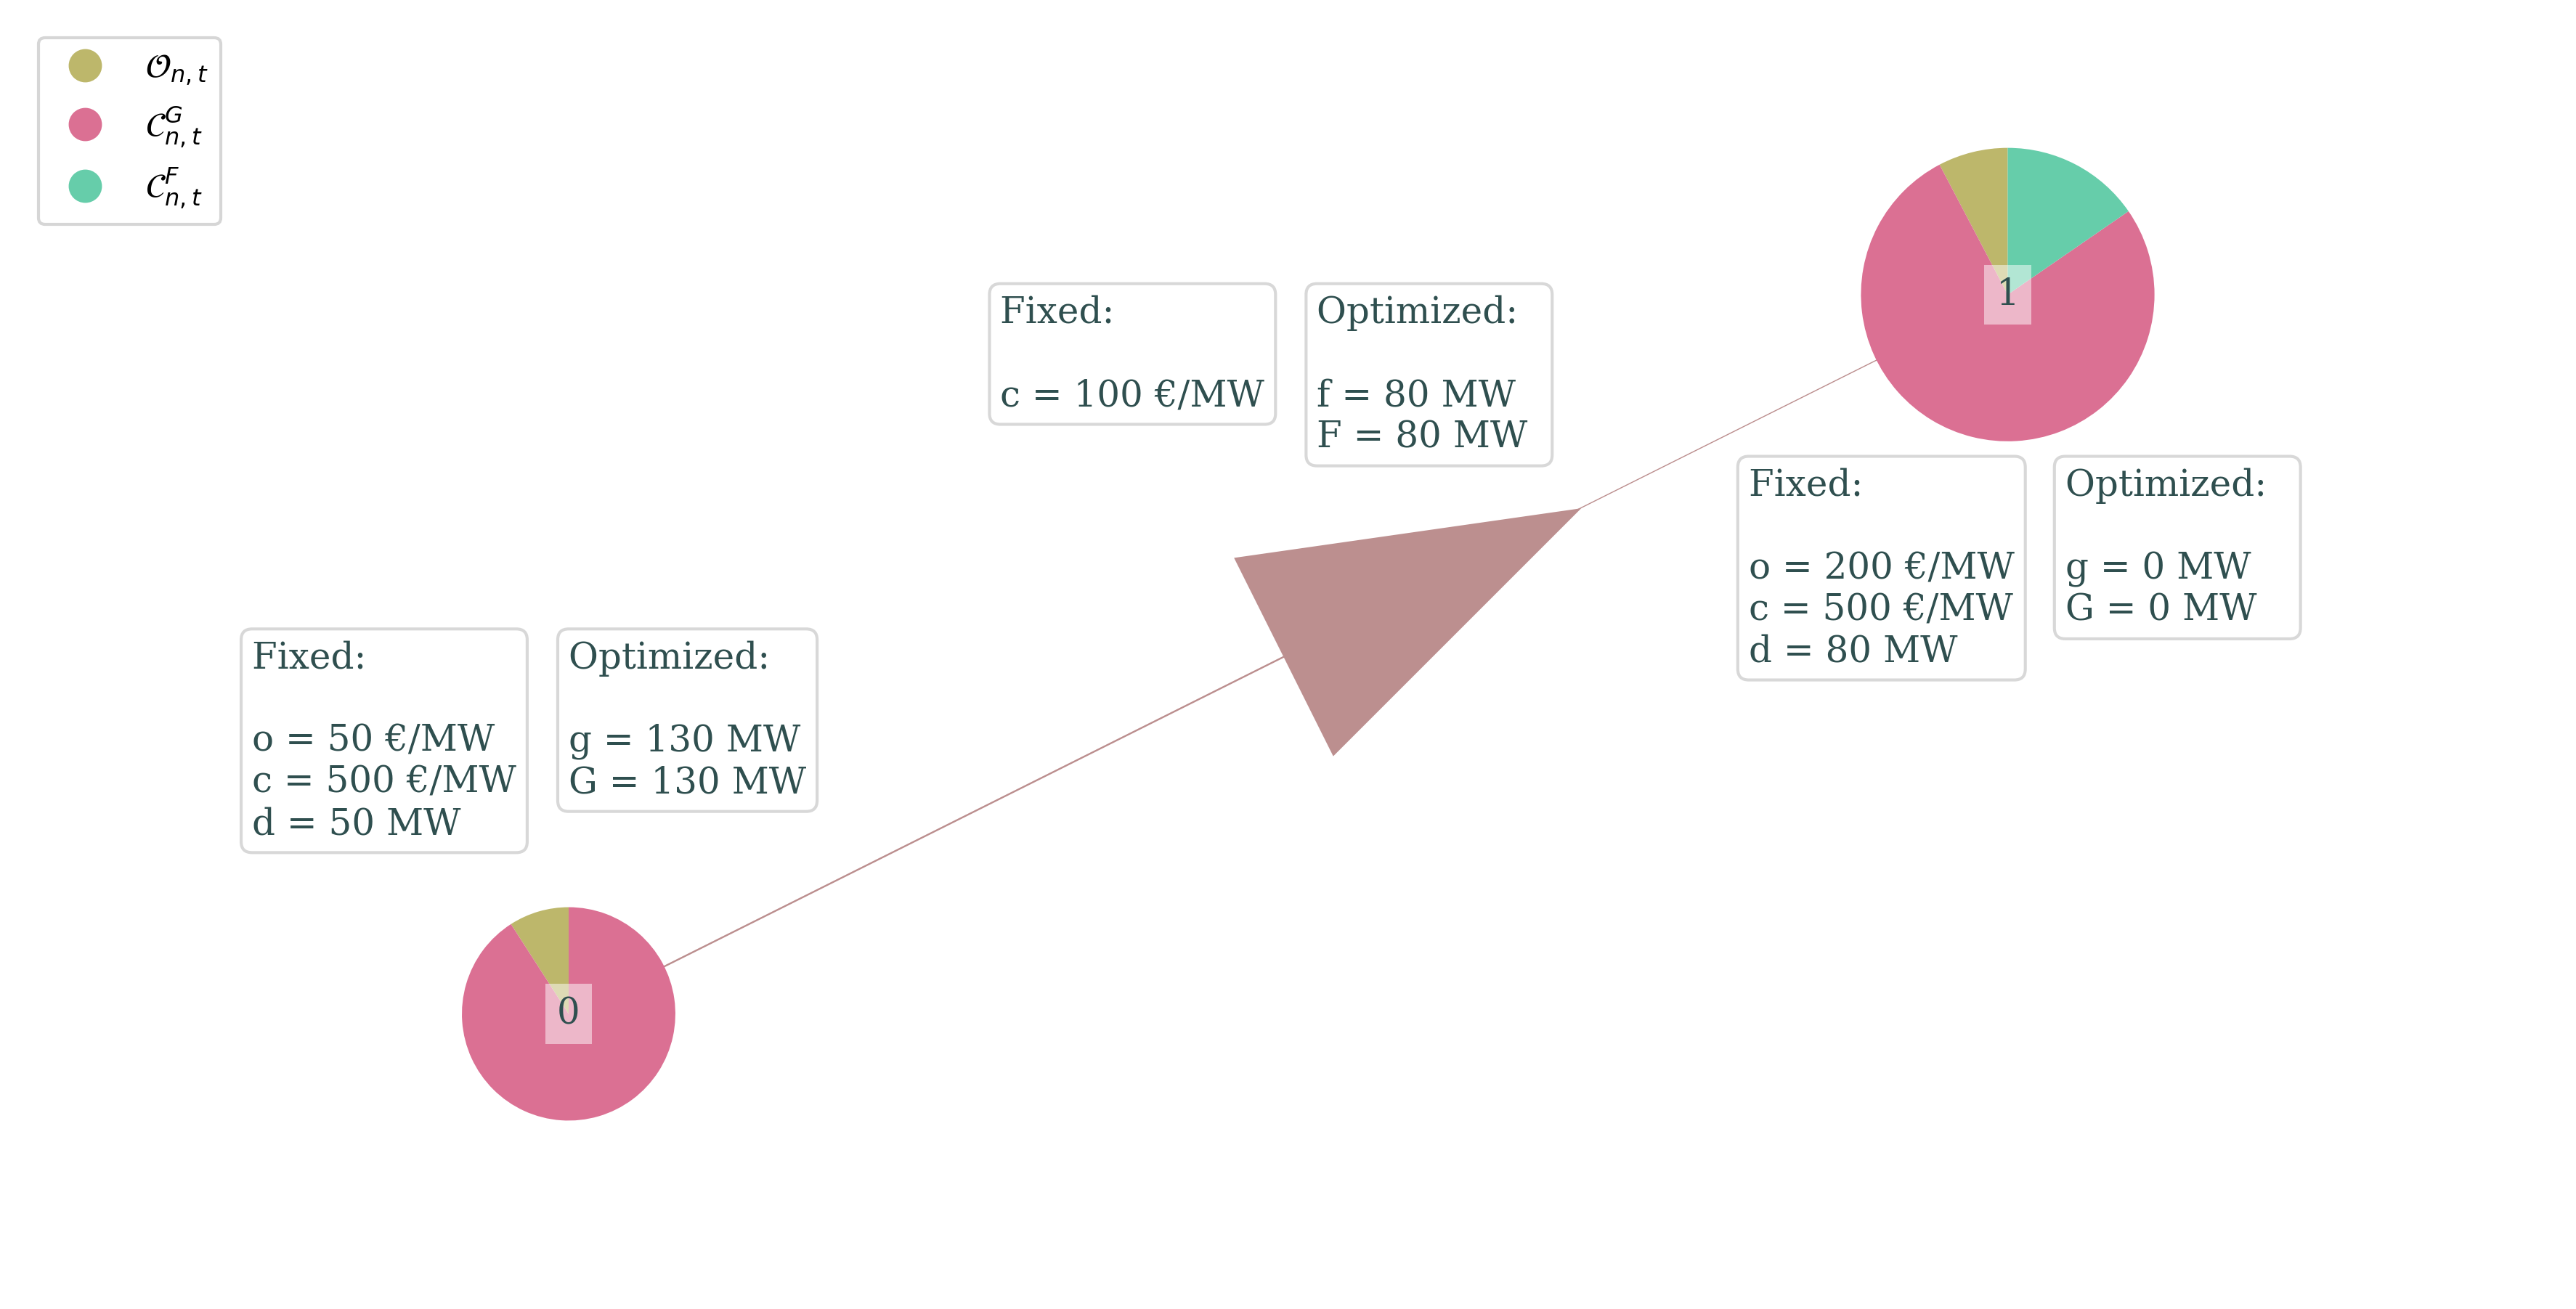
\includegraphics[width=\linewidth]{example_network.png}
 \caption{Illustrative example of a 2-bus network with one optimized time step. Fixed prices and constraining values are given in the left box for each bus and the transmission line. Optimized values are given in the right boxes. Bus~1 has a cheaper operational price $o$, capital prices are the same for both. As both generator capacities are constraint to 100~MW, the optimization also deploys the generator at bus~2. The resulting electricity prices $\lambda$ are then a composition of all prices for operation and capital investments. }
 \label{fig:example_network}
\end{figure*}
The peer-to-peer cost allocation suits for any type of topology and network setup. In the following we showcase a two bus system with one optimized time step and its resulting allocated payments, illustrated in \cref{fig:example_network}. \\

The two buses are connected via one transmission line, each has one generator. Whereas the generator at bus~1 has an operational price of 50 \euro/\megawatthour, the generator at bus~2 has a higher operational price of 200~\euro/\megawatthour. For both the CAPEX rate is set to 500~\euro/MW and the maxmimal capacity is limited to $\capacityGenerationUpper$~=~100~MW. The transmission line has a CAPEX rate of 100~\euro/MW and no upper capacity limit. With a demand of 60~MW at bus~1 and 90~MW at bus~2, the optimization expands the cheaper generator at bus~1 to its full limit of 100~MW. The 40~MW excess power not consumed at bus~1, flow to bus~2 where the generator is built with only 50~MW.  \\
\begin{figure}[h!]
    \begin{subfigure}[c]{\linewidth}
       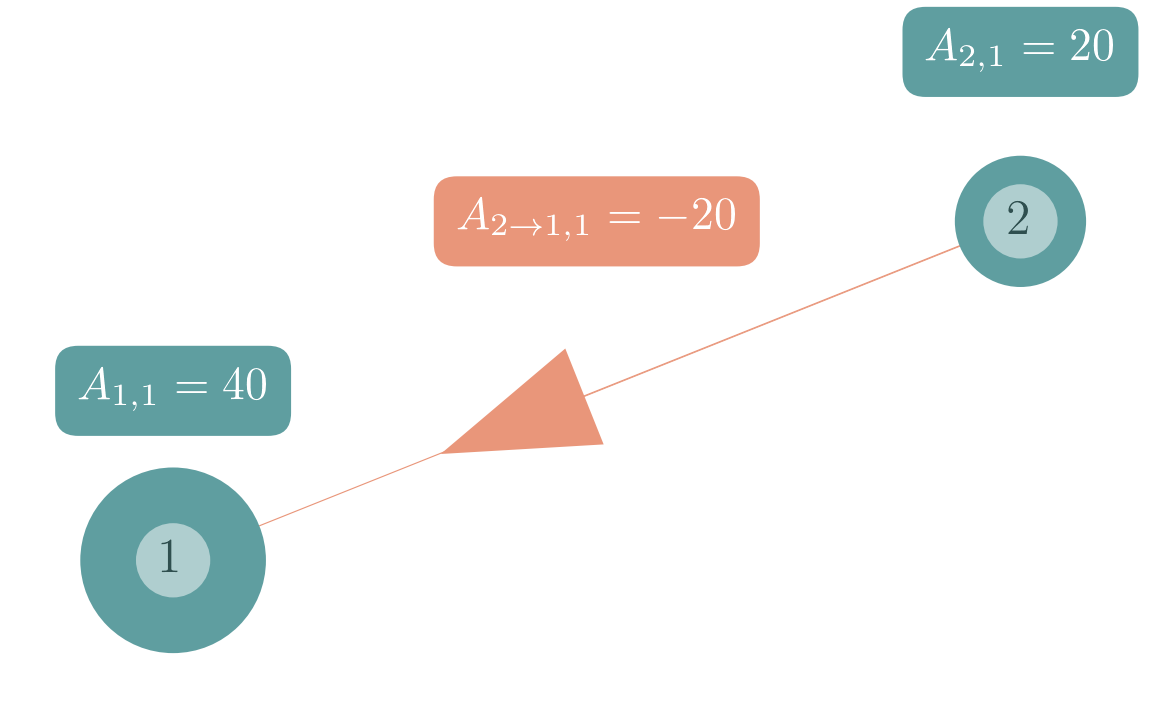
\includegraphics[width=\linewidth]{../figures/example_allocation_bus1.png}
       \vspace{-30pt}
       \subcaption{Allocations to Bus 1}
       \label{fig:example_allocation_bus1}
    \end{subfigure}
    \begin{subfigure}[c]{\linewidth}
       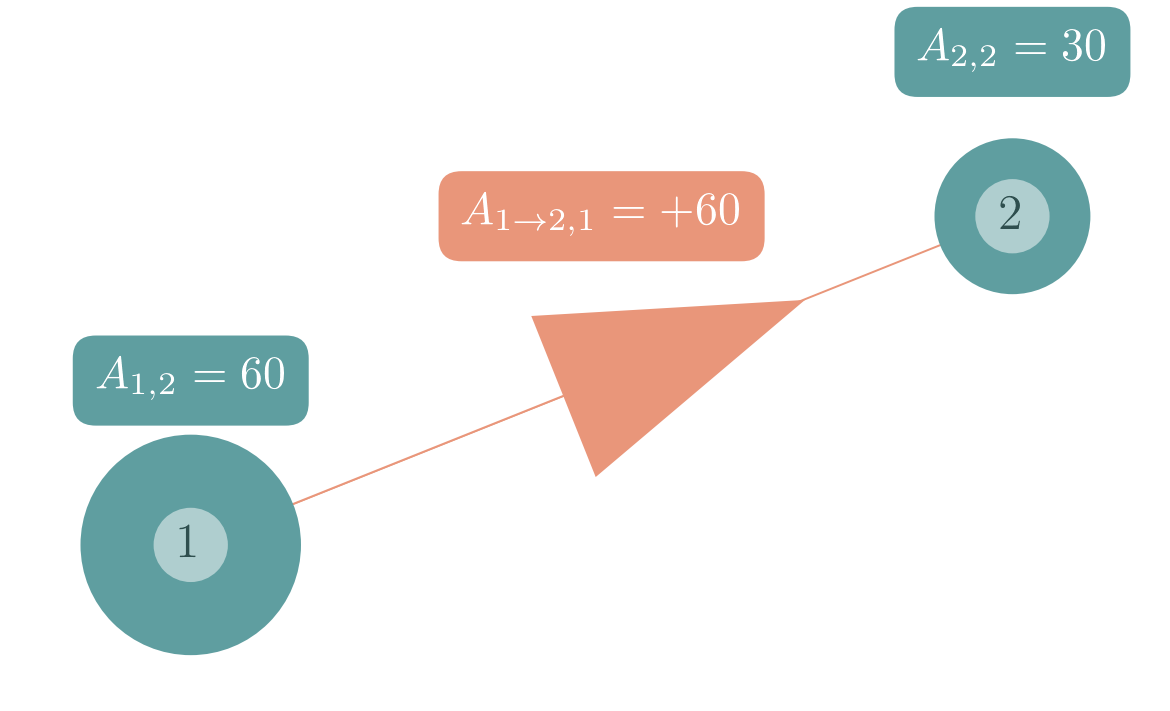
\includegraphics[width=\linewidth]{../figures/example_allocation_bus2.png}
       \vspace{-30pt}
       \subcaption{Allocations to Bus 2}
       \label{fig:example_allocation_bus2}
    \end{subfigure}
	\caption{Full power allocations for the example network in \cref{fig:example_network}. Bus~1 retrieves 40~MW from itself and 20~MW from bus~2. The latter in turn retrieves 60~MW from bus~1 and self supplyies 30~MW. The sum of both net flows equals the resulting flow of $f=40$~MW.}
	\label{fig:example_allocation}
\end{figure}
\begin{figure}[h]
\centering
 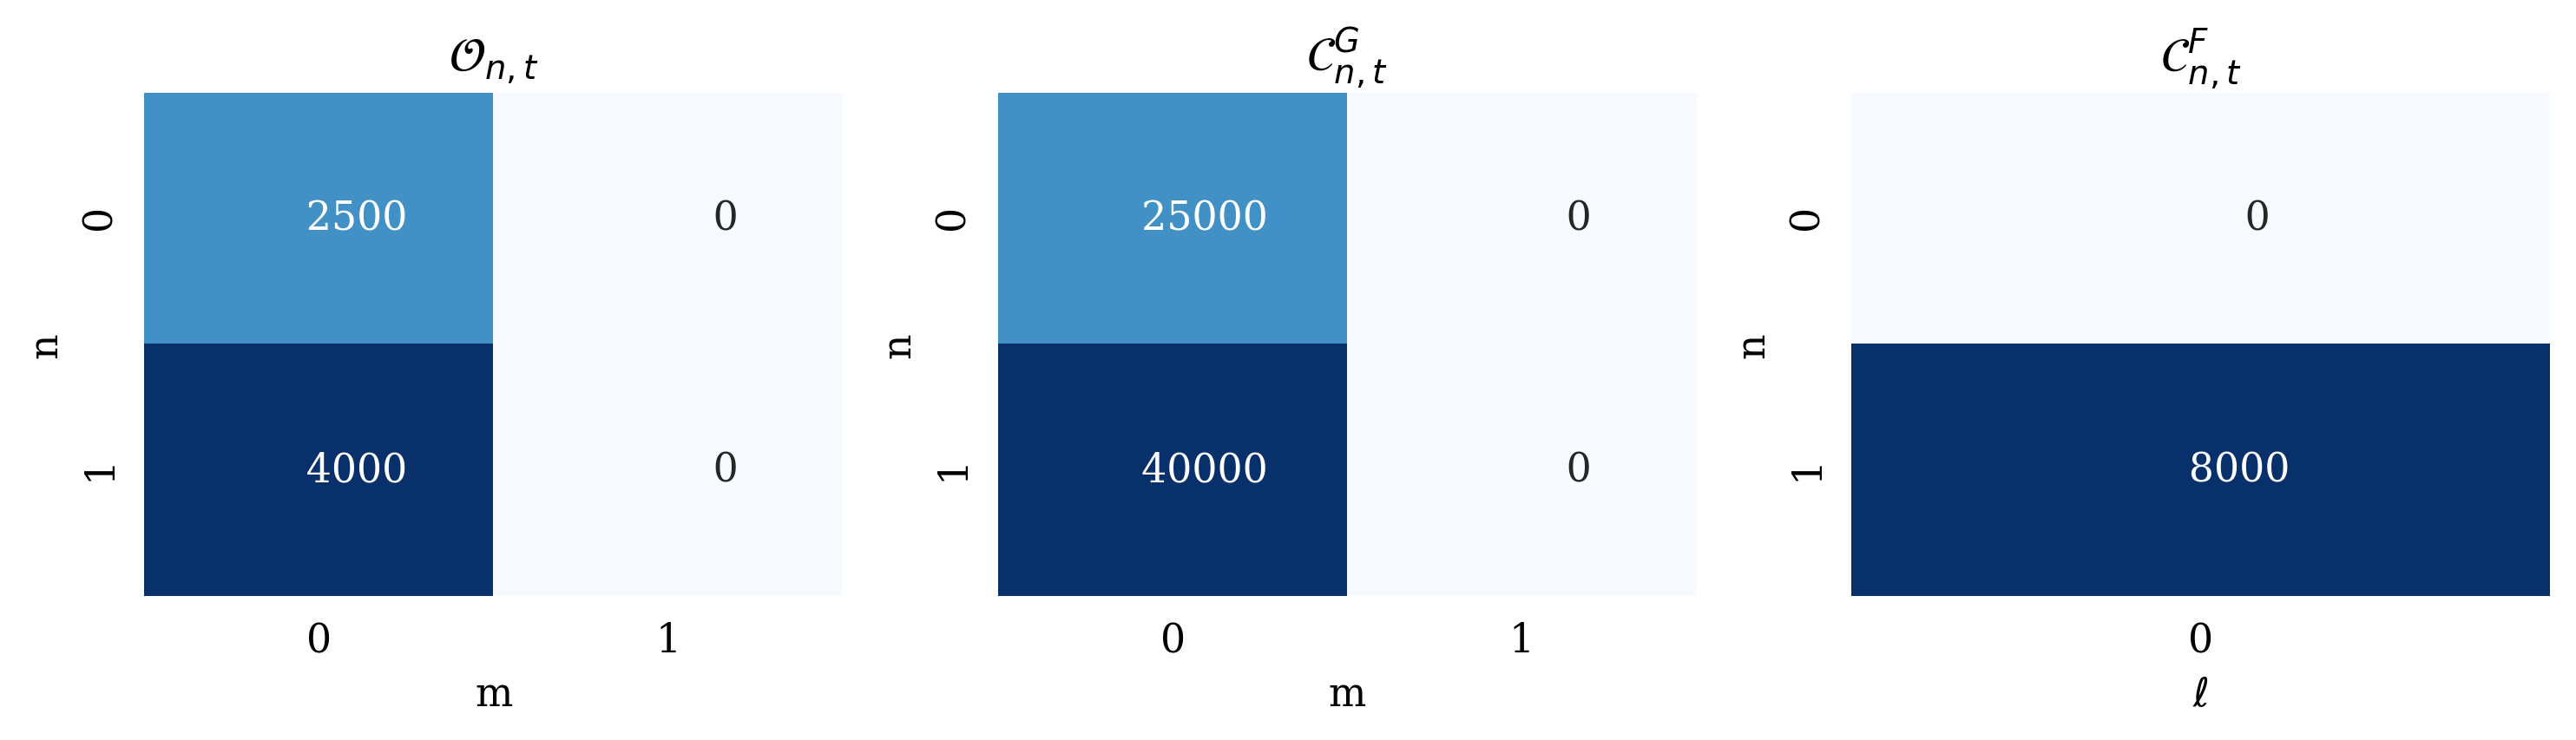
\includegraphics[width=\linewidth]{example_payoff.png}
 \caption{Full cost allocation for the example setup shown in \cref{fig:example_network}. The payments are derived on the basis of \cref{eq:allocate_opexGeneration_detailed,eq:allocate_capexGeneration_detailed,eq:allocate_capexFlow_detailed}. Consumers at bus $n$ have to pay each generator proportional to their consumption. As we only consider one time step the proportionality applies for OPEX $\mathcal{O}_n$ and CAPEX $\mathcal{C}_n$. As bus~1 induces a relieving flow an line~1 and therefore ``prevents`` further tranmission expansion, it is rewarded proportional to the relief.}
 \label{fig:example_payoff}
\end{figure}
\Cref{fig:example_allocation} shows the allocated transactions for both buses 1~\&~2 separately. The resulting peer-to-peer payments are given in \cref{fig:example_payoff}.
The upper graph \cref{fig:example_allocation_bus1} shows that $A_{1,1}=40$~MW at bus~1 are self-sustained. Consumers at bus~1 consequently pay 2k~\euro~OPEX and 22k~\euro~CAPEX to the generator at bus~1. The missing 20~MW in order to supply $d_1$ come from bus~2 and induce a subflow on line 1 of $A_{2 \rightarrow 1, 1} = -20$. As this flow is in contrary direction to the total flow, it is relieving the transmission system. This translates to a congestion reward for consumers at bus~1 of $c_{\ell=1} A_{2 \rightarrow 1, 1}$~=~2k~\euro\, which is exactly the cost that had to be spent on the transmission system if bus~1 didn't induce a relieving flow. 

The lower graph \cref{fig:example_allocation_bus2} illustrates the impact of consumption at bus~2. As $d_2$ is higher than $d_1$ the retrievements from both generators are proportionately increased as well as the OPEX and CAPEX allocations to the generators, see \cref{fig:example_payoff}. But instead of a relieving flow, consumers at bus~2 drive the burdening flow in direction of congestion. Hence the payoff to the transmission system is positive and much higher than for bus~1.

The sum of all rows in the payoff matrix in \cref{fig:example_payoff} yields the revenues of the assets $m, \ell$. These values match their overall spendings, \textit{e.g.} the total revenue of the transmission line is 4k~\euro\, which equals the cost for investments $c_{1}\,F_{1}$. The sum of all columns yields the total payment of consumers at bus $n$. For example the sum of payments of bus~1 is 36k~\euro. This is exactly the electricity price of 600~\euro/MW times the consumption of 60~MW, $\lambda_1 d_1$. 

The fact that OPEX and CAPEX allocations are proportional to the total consumption at a bus... 


% \bibliographystyle{ieeetr}
\printbibliography

\clearpage
\appendix

\section{Appendix}

\subsection{\texorpdfstring{Proof \Cref{eq:allocate_peer}}{First Proof}}
\label{sec:proof_allocate_peer}

\Cref{eq:allocate_peer} follows from summing $\allocateTransaction$ over all incoming flows to $n$ and taking into account the power that $n$ provides by itsself, $\slackk \, \nodaldemand$, which leads us to
\begin{align}
 \allocatePeer &= \slackk \, \nodaldemand - \sum_{\ell} \incidence \, \allocateTransaction \\
 &= \slackk \, \nodaldemand - \sum_\ell \incidence \left(  \ptdfEqual[m] - \ptdfEqual \right) \slackk[m] \, \nodaldemand  \\
 &= \slackk \, \nodaldemand - \left(  \delta_{n,m} - \dfrac{1}{N} - \delta_{n,n} + \dfrac{1}{N} \right) \slackk[m] \, \nodaldemand  \\
 &= \slackk \, \nodaldemand - \left(  \delta_{n,m} - 1 \right) \slackk[m] \, \nodaldemand  \\
 &= \slackk[m] \, \nodaldemand 
\label{eq:proof_allocate_peer}
\end{align}
where we used \cref{eq:slack} and the fact that the equally distributed slack amounts to $1/N$ for all N nodes in the network. 



\subsection{\texorpdfstring{Proof of \Cref{eq:sum_n_allocate_peer}}{Second proof}}
\label{sec:proof_sum_n_allocate_peer}
The relation follows from multiplying \cref{eq:flow_from_demand} with $\sum_m \incidence[m]$, and solving for $\allocatePeer$
\begin{align}
\sum_m \incidence[m] \, \flow &= - \sum_{m,n} \incidence[m] \, \ptdf \, \nodaldemand \\
\nodalgeneration[m] - \nodaldemand[m] &= - \delta_{m,n} \, \nodaldemand + \slackk[m] \, \nodaldemand    \\
\allocatePeer &= \nodalgeneration[m] - \nodaldemand[m] + \delta_{m,n} \nodaldemand \\
\sum_n \allocatePeer &= \nodalgeneration[m]
\end{align}



\subsection{\texorpdfstring{Solution Space of $\boldsymbol{\slackk[m]}$}{Solution Space of the Slack}}
\label{sec:solution_space_of_the_slack}

All choices of $\slackk[m]$ fulfilling \cref{eq:flow_from_demand} determine the solution space of $\slackk$. In the $N \times N$ nodal space this translates to the constraint given by \cref{eq:sum_n_allocate_peer} which denotes
\begin{align}
 \nodalgeneration[m] = \sum_n \slackk[m] \, \nodaldemand  
 \label{eq:solution_space_slack}
\end{align}
Solving for $\slackk[m]$ directly leads to 
\begin{align}
 \slackk[m] = c \, \generation[m] 
\end{align}
where $c$ is the inverse of the total consumption or production $c = 1 / \sum_n \nodaldemand   = 1 / \sum_n \nodalgeneration$. \\
However \cref{eq:solution_space_slack} has an inherent degree of freedom and can be reformulated as 
\begin{align}
 \nodalgeneration[m] = \sum_n \Slackk \, \nodaldemand  
 \label{eq:solution_space_slack_extended}
\end{align}
where $\Slackk$ denote the individual choice of slack for each bus $n$. For example the Marginal Participation cite[] algorithm takes only net injections into account. This sets the individual slack to 
\begin{align}
\Slackk &= \dfrac{ \delta_{m,n}\,\selfconsumption[m] + \gamma_t \, \netconsumption  \, \netproduction[m]}{\nodaldemand}
\end{align}
where 
\begin{itemize}
%  \item $\injection = \left( \nodalgeneration - \nodaldemand \right) $ denotes the nodal injection
 \item $\netproduction = \text{min}\left( \nodalgeneration - \nodaldemand , 0 \right) $ denotes the nodal net production 
 \item $\netconsumption = \text{min}\left( \nodaldemand  - \nodalgeneration, 0 \right)$ denotes the nodal net consumption
 \item $\selfconsumption = \text{min}\left( \netproduction, \netconsumption \right)$ the denotes  nodal self-consumption. That is the power generated and at the same time consumed at node $n$ and 
 \item $\gamma_t = \dfrac{1}{\sum_n \netproduction} = \dfrac{1}{\sum_n \netconsumption}$ is the inverse of the total injected/extracted power at time $t$.
\end{itemize}







\end{document}
